\documentclass{article}
\setlength{\parskip}{5pt} % esp. entre parrafos
\setlength{\parindent}{0pt} % esp. al inicio de un parrafo
\usepackage{amsmath} % mates
\usepackage[sort&compress,numbers]{natbib} % referencias
\usepackage{url} % que las URLs se vean lindos
\usepackage[top=25mm,left=20mm,right=20mm,bottom=25mm]{geometry} % margenes
\usepackage{hyperref} % ligas de URLs
\usepackage{graphicx} % poner figuras
\usepackage[spanish]{babel} % otros idiomas
\usepackage[utf8]{inputenc}
\author{Jesus Alberto Funes Mendoza  \\
Melissa Lizeth Galindo Reyes  \\
Ramón Samuel Blanco Ramirez  \\
Aída Mata Moreno  \\
Miriam Itzel Mata Porras  \\ 
Victor Adrían Higuera Vázquez} % author
\title{Actividad 2: Prótesis de Mano} % titulo
\date{\today}
\usepackage{float} 
\begin{document} % inicia contenido

\maketitle % cabecera

\begin{abstract} % resumen
Las prótesis en las manos, son muy importantes hoy en día, ya que les ayuda en dado caso que haya una ausencia de la mano, cada año la tecnología nos ayuda poder actualizar las prótesis, para poder así que esta sea más fácil de manejarla, todo esto conlleva en muchos procesos, como lo son los mecanismos y el estudio de como nuestro cuerpo y cerebro responden a cada una de ellas. 
\end{abstract}

\section{Introducción}\label{intro} % seccion y etiqueta

 
Una prótesis es una extensión artificial que reemplaza una parte faltante del cuerpo. Las hay de dos tipos, pasivas y activas; las primeras también suelen ser llamadas cosméticas ya que no tienen movimiento propio y su función es puramente estética, lás prótesis activas se clasifican a su vez en mecánicas, eléctricas, neumáticas, mioeléctricas e híbridas. Las mioeléctricas se pueden dividir en sistema de actuación, de transmisión, de control y de suspensión (Figura 1)\cite{ff2}. 

\begin{figure}[H] % figura
    \centering
    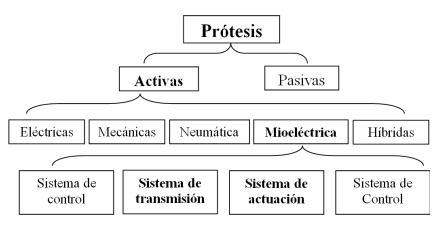
\includegraphics[width=100mm]{Clasificaciones.png} % archivo
    \caption{Clasificaciones de prótesis\cite{ff2}.}
    \label{grafica}
\end{figure}


\section{Desarrollo}
\subsection{Anatomía de la mano}
La mano está compuesta de diferentes huesos, músculos, y ligamentos que permiten una gran cantidad de movimientos y destrezas. Existen tres principales tipos de huesos en la mano, entre los cuales se incluyen: 

\begin{figure}[H] % figura
    \centering
    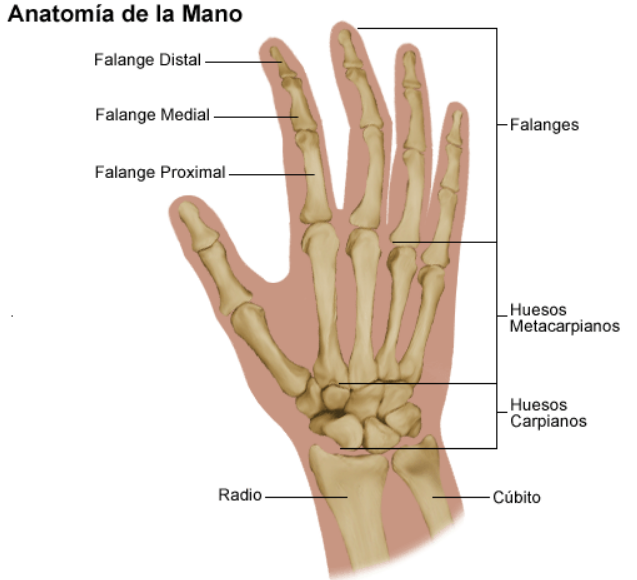
\includegraphics[width=100mm]{mano.png} % archivo
    \caption{Anatomía de la mano\cite{ff3}.}
    \label{grafica:dos}
\end{figure}

Falanges: Los 14 huesos que están en los dedos de cada mano y también en los dedos de cada pie. Cada dedo tiene tres falanges (distal, media y proximal); solamente el pulgar tiene dos\cite{ff3}. 

Huesos metacarpianos: Los cinco huesos que componen la parte media de la mano\cite{ff3}. 

Huesos carpianos: Los ocho huesos que forman la muñeca. Los huesos carpianos están conectados a dos huesos del brazo--el hueso cúbito y el hueso radio\cite{ff3}. 

En la mano se pueden encontrar numerosos músculos, ligamentos, y vainas. Los músculos son estructuras que se contraen y permiten el movimiento de los huesos de la mano. Los ligamentos son tejidos fibrosos que ayudan a unir las articulaciones de la mano. Las vainas son estructuras tubulares que rodean parte de los dedos\cite{ff3}. 

\subsection{¿Cómo funciona la prótesis de una mano?}
Las prótesis mioeléctricas son sistemas accionados por servomotores, estos son controlados por señales electromiografías superficiales (EMGS), las cuales son intramusculares; existen sensores que pueden ser mediante agujas o electrodos colocados en el muñón del paciente, permitiéndoles de este modo capturar la señal superficialmente. Al estudio que se genera a la actividad eléctrica de los músculos se le denomina electromiografía. La contracción generada al cerrar la mano es mediante células que son activadas neurológicamente y se produce la señal eléctrica por la excitación expuesta en estas. Para concluir con este apartado se describe una de las manos más avanzadas desarrollada por investigadores del Instituto de Robótica y Mecatrónica del Centro Aeroespacial alemán, esta mano puede absorber altos impactos, tomando como ejemplo el ser golpeado con un bate de beisbol. Cuenta con 19 grados de libertad y es capaz de ejercer una fuerza de 30 Newtons\cite{ff4}   

El control mioeléctrico es considerablemente el esquema de control más popular. Se desarrolla en el concepto de que siempre que un músculo en el cuerpo se contrae o se flexiona, se produce una pequeña señal eléctrica (EMG) que es creada por la interacción química en el cuerpo. Esta señal es demasiado pequeña (5 a 20 µV) Un micro-voltio es una millonésima parte de un voltio. Para poner esto de una forma más entendible, una bombilla eléctrica típica usa 110 a 120 voltios, de forma que esta señal es un millón de veces más pequeña que la electricidad requerida para alimentar una bombilla eléctrica\cite{ff4}   

El uso de sensores llamados electrodos que entran en contacto con la superficie de la piel permite registrar la señal EMG. Una vez registrada, esta señal se amplifica y es procesada después por un controlador que conmuta los motores encendiéndolos y apagándolos en la mano, la muñeca o el codo para producir movimiento y funcionalidad\cite{ff4}. 

\begin{figure}[H] % figura
    \centering
    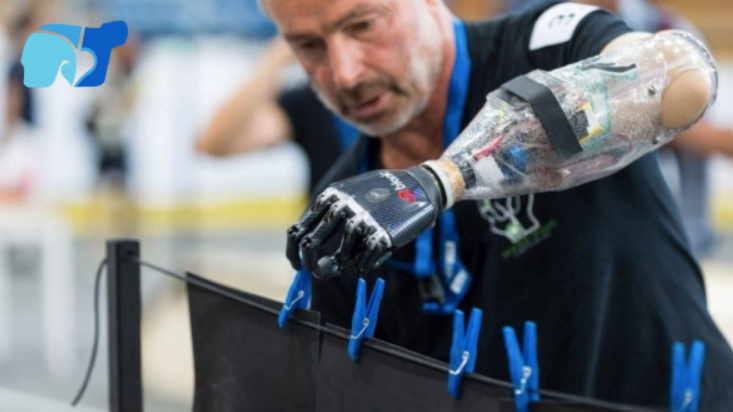
\includegraphics[width=100mm]{representacion.png} % archivo
    \caption{Representación de una prótesis de brazo\cite{ff4}.}
    \label{grafica:tres}
\end{figure}

Éste tipo de prótesis tiene la ventaja de que sólo requieren que el usuario mueva sus músculos para operarla, a diferencia de las prótesis que son manipuladas por el miembro y que requieren el movimiento general del cuerpo. Una prótesis controlada en forma mioeléctrica también elimina el arnés de suspensión usando una de las dos siguientes técnicas de suspensión: bloqueo de tejidos blandos-esqueleto o succión\cite{ff4}. 



\subsection{Sistema de actuación} 
El sistema de actuacion está compuesto básicamente por los elements encargados de producir la potencia mecánica del sistema, estos eleentos son comúnmente llamados actuadores, que son disposiivos capaces de generar una fuerza apartir de líqudo , energía eléctrica o gaseosa\cite{ff2}. 


En la actualidad se han propuesto algunos sitemas de actuación para las prótesis comerciales, prototipos en desaroolo y manos robótixas antropmórfica. Estos sistemas se diferencian unos de otros no sólo en el principio de funcionamiento, ya que hay factores muy relevantes como el ruido, cantidd de energía consumida, tamaño, peso, eficiencia, potencia alcanzada, entre otros\cite{ff2}. 

Los actuadores eléctricos son los más amplicamente usados por los diseñadores de prótesis de mano porque presentan una serie de ventajas sobe los otros tipos de actudores, como alta eficiencia, gran disponibilidad y los tamaños compactos\cite{ff2}.

Algunas de las ventajas de este tipo de motores son el buen rendimiento y fiabilidad, bajo costo, respuesta rápida. Por otro lado producen fricción y por consecuencia calor y ruido, generan chispas\cite{ff2}. 

Los motores CD son utilizas en proyectos como "CyberHand" y "RTR II" desarrollados en la Scuola Superiore Sant'Anna; "TBM Hand" de la Universidad de Toronto; "SensorHand" de Otto pck, "MYO Electric Hand" de Centri\cite{ff2}. 

\begin{figure}[H] % figura
    \centering
    \includegraphics[width=100mm]{Prótesis.png} % archivo
    \caption{Algunas prótesis que utilizan motores CD\cite{ff2}.}
    \label{grafica:cuatro}
\end{figure}

Los servomotores son otro tipo muy común de actuadores, a grandes rasgos consiste en un motor CD, que permite situar el eje de salida en una determinada posición angular, mediante una señal externa de control. Está fromado pr carcasa, motor, engranes que reducen la velocidad del motor y aumentan el par de salida, circuito electrónico que controla la posición de salida, potenciómetro que se utiliza como sensor para concocer la posición del eje de salida. Por lo genereal un servomotor puede girar aproximadamente 180 grados\cite{ff2}. 

Las ventajas que presenta son: relativamente fácil de controlar, puede ser conectado directamente a microcontroladores, su eje puede ser llevado a una posición especifica, es eficiente. Sin embargo, algunas de sus desventajas son: que no gira de manera continua, para evitar interferencia en los circuitoselctrónicos es conveniente conectar la alimentación de los servomotores a una fuente diferente a la usada para los circuitos de control\cite{ff2}. 

Son utilizados en el camplo de las prótesi en proyectos como "Gifu Hand" de la Universidad de Gifu en Japón. Desafortunadamente, al utilizar este tipo de motores se requiere que el movimiento completo del dedo se puede realizar con el giro de 180° del eje de salida del servomotor. Cuando se utiliza este actuador ya no es necesario un sistema de reducción de velocidad\cite{ff2}. 

También, dentro de los motores encontrados a los ultrasónicos, en particular a los rotativos onda viajera, que son motores eléctricos formados principalmente pr 4 componentes (rotor, estator, electrodo y material piezoeléctrico). El elemento encargado en generar las microdeformaciones a partir de un nivel de voltaje es el material piezoeléctrico , éste se encuentra adherido a un electrodo que se encarga de trasmitir las señales de excitación, estos dos componentes se acoplan al estator que trasmitirá el movimientos por fricción al rotor. El principio de funcionamiento de los motores ultrasónicos de onda viajera es el de crear un movimiento elíptico enel punto de contacto entre el rotor y el estator que da lugar al movimiento del motor. Sus ventajas son: elevado par a bajas velocidades. rápida respuesta y uena parada con los que se logra una buena controlabilidad, funcionamiento silencioso, estructura simple, no le afectan campos magnéticos externos ni los genera, eficienia insensible a la miniaturización, Sin embargo, sus principales descentajas son: necesita un suministro de potncia de alta frecuencia, bajo tiempo de vida útil debido a la alta fricción entre el estator y el rotor y la caída en las características par-velocidad con el tiempo\cite{ff2}. 

Estos motores son usados como actuadores  proyectos como "Utah Arm" de la empresa Motion Control y "MANUS Hand", la primera es una prótesis existente en el mercado y la segunda fue desarrollada como una mano robótica antromórfica. El uso de motores ultrasónicos en prótesis ha tenido poca aceptaicón entre los diseñadores debido principalmente a que tienen que ser alimentados por una fuente de portencia de alta precuencia, y algo que hasta la fecha es limitado es la cantidad de energía que puede ser almacenada en las baterías que llevan las prótesis\cite{ff2}. 

\begin{figure}[H] % figura
    \centering
    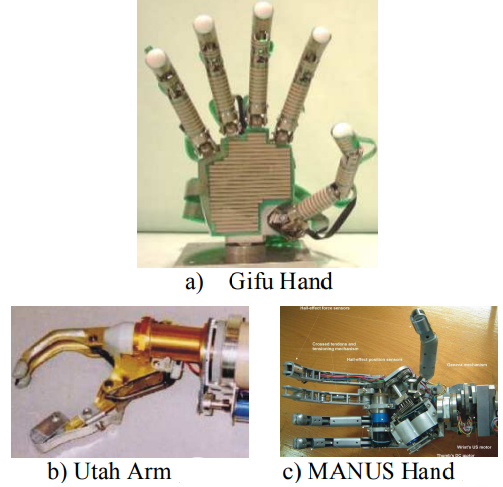
\includegraphics[width=100mm]{Protesis 2.png} % archivo
    \caption{Prótesis que utilizan como actuadores a) servomotores, b) y c) motores ultrasónicos\cite{ff2}.}
    \label{grafica:cinco}
\end{figure}

En los motores sin escobillas, a diferencia de los que pasa en un motor CD convencional, los electroimanes no se mueven, en lugar de eso, ls magnetos permanentes rotan y la armadura permnece estática. La mayor ventaja es que al no haber rozamiento entre los magnetos permanentes y la armadura genera menos calor y por lo tanto hay menor perdida de fricción, mayor vida útl, mayor eficiencia, menos peso y no produce chispas. Los proyectos más sobresalientes que hacen uso de este tipo de motores son "DLR Hand" del Centro Alemán de Investigaciones Aeroespaciales, "DLR/HIT Hand" del Centro de Investigaciones Aeroespaciales en conjunto con el Instituto de Tecnología de Harbin, China, y "Robonaut Hand" de la NASA\cite{ff2}. 

En los últimos años se ha incrementado el uso de actuadores no convencionales, como en el caso de las aleaciones con memoria de forma (SMA), ue se puede considerar como actuadores eléctricos debido a que utilizan de este tipo de energía para su funcionamiento. Son aleaciones metálicas a las cuales estando a temperatura relativamnte fría se deforman mediante la accion de una carga externa,una vez retirada la carga puede regresar a la forma que tenían originalmente mediante un simple calentamiento (generalemnte se hace pasar una corriente eléctrica). Las ventajas más significativas que presenta cuando son utilzadas en prótesis son: la generación de movimientos lineales, actuador muy ligero, pueden ser manufacturadas en casi culquier forma y tamaño, tienen un alto nivel de recuperación plástica, resisten la corrosión y son estables frentea aplicaciones cíclicas. En cambio se requiere el manejo de temperaturas altas, tiene movimientos poco precisos, falta de control en el tiempo de enfriado y su eficacia energética es baja. Este actuador es utilizado en la "SBC Hand" del Instituto Tecnológico de Massachusetts\cite{ff2}. 


\begin{figure}[H] % figura
    \centering
    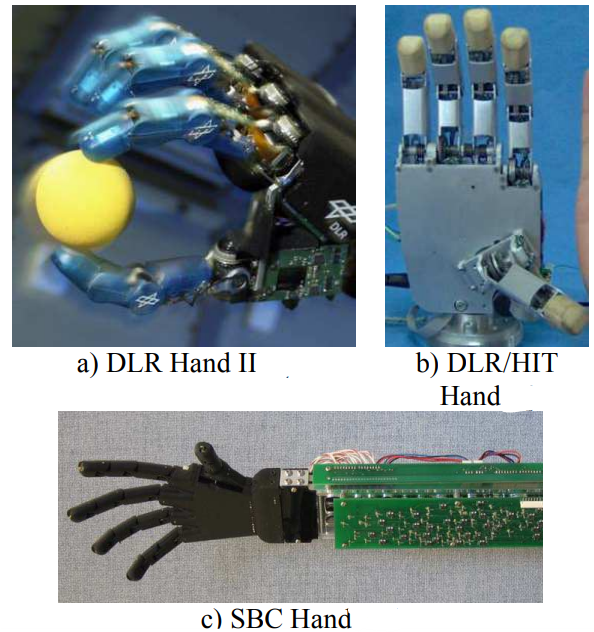
\includegraphics[width=100mm]{protesis 3.png} % archivo
    \caption{Manos que utilizan como actuadores a) y b) motores sin escobillas, c) SMA\cite{ff2}.}
    \label{grafica:seis}
\end{figure}


Otro de los grandes campos son los actuadores neumáticos, que por sus características no son tan usados para la generación de potencia en prótesis ya que presentan una serie de desventajas. Uno de estos actuadores es el llamado "músculo neumático" que consiste en un tubo de goma cubierto por una red de pláctico acomodada en forma de tijera (trenzada), cuando es inflado con aire comprimido a baja presión acorta su longitud ejerciendo una fuerza en ambos extremos del tubo. Algunas de las ventajas que presenta son el bajo peso, , gran flexibilidad, ofrece movimiento lineal, las desventajas prinicplaes cuando se emplea en prótesis son un difíci control, requiere de un sistema de compresión de aire además del riesgo de posibles fugas de fluido. Los músculos neumáticos se han empleado en proyectos como "Blackfingers" desarrollado en Politécnico de Milano; y "Shadow Hand" de la Shadow Robot Company, ambosn desarrollados como manos robóticas. Con est tipo de actuadores se puede lograr movimientos suaves algo deseado por diseñadores de prótesis, aunque su implementación no se ha dado debido a las obvias razones del peso y volumen del siste de compresión de aire, ya que una de las principales cosas a tener en cuenta es el diseño de prótesis  es el peso de ésta, en vista de que el paciente tiene que cargarla la mayor parte del día\cite{ff2}. 

Finalmente encontramos a los actuadores hidráulicos, que dentro del campo de las prótesis de mano son escasamente utilizados. El único proycto que a la fecha los utiliza es "FluidHand" desarrollado en la universidad de Karlsruhe que ha desarrollado a la medida tanto su bomba hidráulica de engranes externos como sus electroválvulas. La desventaja más clara  es la necesidad de un sistema de bombeo, en cambio puede proporcionar movimiento lineales y suaves. A diferencia de los actuadores neumáticos, los hidráulicos tienen mejor futuro como mecanismos de deneradores de potencia porque ocupan menos espacio y se puede lograr más potencia. Desafortunadamente los elementos existentes en el mercado como bombas y electroválvulas aun son demasiado grandes para ser utilizados, por lo que es necesario realizar el diseño a la medida, como es el caso de la FluidHand\cite{ff2}.  

\begin{figure}[H] % figura
    \centering
    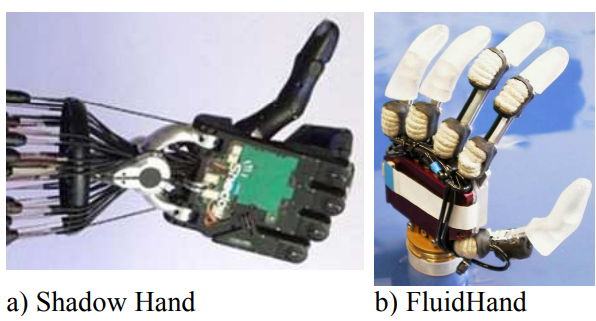
\includegraphics[width=100mm]{protesis 4.png} % archivo
    \caption{Manos que utilizan energía neumática a) e hidráulica b)\cite{ff2}.}
    \label{grafica:siete}
\end{figure}

\subsection{Metodología del diseño de una prótesis de mano}

\textbf{Diseño y simulación de prótesis de mano} 

La importancia del desarrollo de una prótesis mioeléctrica radica en que esta permitirá a un sector significativo de la población afectada de amputación, acceder a un dispositivo funcional que les brindará autonomía, mejorará sustancialmente su calidad de vida, su autoestima y aumentará sus probabilidades de reinserción a la sociedad como una persona útil a la misma.
Por otra parte, debido a que un producto como este requiere de la utilización de alta tecnología, en especial dentro de los procesos de fabricación y ensamble, la investigación pretende determinar si es posible implementar una estrategia de producción que sea aplicable en países no desarrollados ampliamente en la industria, ya que una de las limitantes de la industria en estos países es su poca capacidad para generar propuestas innovadoras hacia el mercado interno y externo que sean posibles de desarrollar utilizando la tecnología que en la actualidad está instalada. Al posibilitar la fabricación de la prótesis en estos países, los costos sobre sus usuarios finales se reducirán significativamente y esto facilitaría su acceso a un dispositivo con mayor funcionalidad, mejor apariencia y la industria se vería beneficiada con un desarrollo a nivel tecnológico que aportará estrategias para aprovechar mejor la capacidad de producción actual\cite{ff5}.


\textbf{Definición de los requerimientos del cliente.} 


Metodología:
\\1. Recopilar los datos del cliente, sin procesar.
\\2. Interpretar estos datos en términos de las necesidades del cliente.
\\3. Organizar las necesidades en una jerarquía: a) primarias, b) secundarias y en caso de
que existan, c) terciarias.
\\4. Establecer que tan importantes relativamente son estas necesidades. 
\\5. Analizar y reflexionar sobre los resultados arrojados por el proceso\cite{ff5}.


\textbf{Especificaciones de ingeniería.} 


Metodología:
\\1. Elaborar una lista de métricas.
\\2. Recabar información de comparaciones con la competencia.
\\3. Establecer valores objetivos ideales y marginalmente aceptables.
\\4. Reflexionar en los resultados y el proceso\cite{ff5}.

\begin{figure}[H] % figura
    \centering
    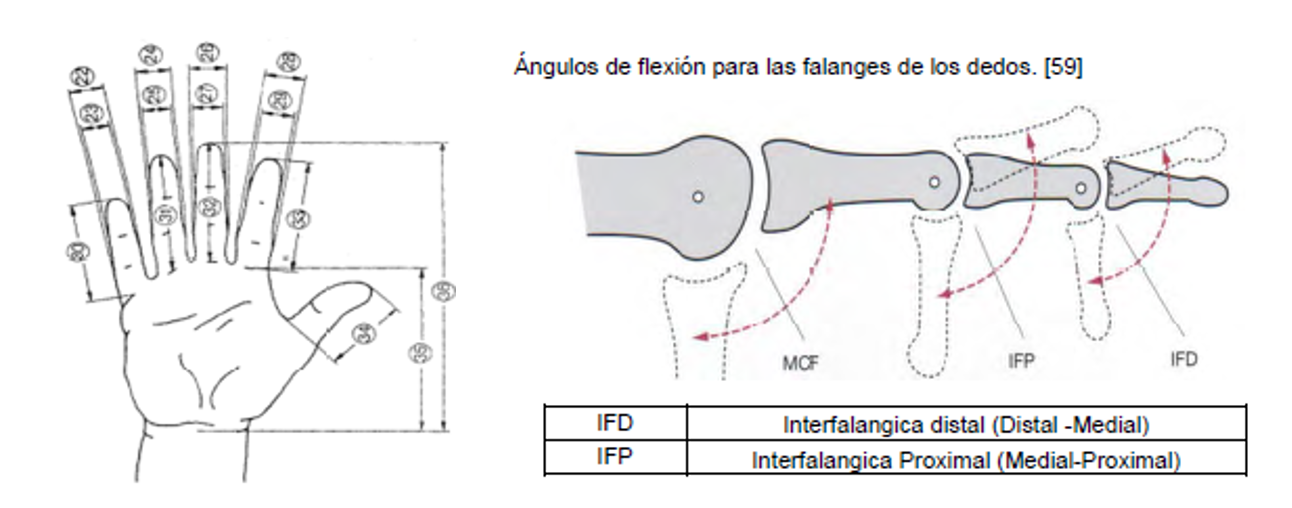
\includegraphics[width=100mm]{anatomia y mecanida de movimiento.png} % archivo
    \caption{Anatomía y mecánica de movimiento de la mano)\cite{ff5}.}
    \label{grafica:ocho}
\end{figure}

\textbf{Diseño conceptual} 

1)	Aclarar el problema:

a)	Entenderlo.
\\b)	Descomponerlo
\\c)	Enfocarse en subproblemas críticos.


2)	Búsqueda externa de soluciones:
\\a)	Usuarios Líderes.
\\b)	Expertos.
\\c)	Patentes.
\\d)	Literatura.
\\e)	Benchmarking.


3)	Búsqueda interna de soluciones:
\\a)	Individual.
\\b)	En grupo.


4)	Exploración sistemática:
\\a)	Árbol de clasificación
\\b)	Tabla de combinación.


5)	Reflexión sobre las soluciones propuestas y el proceso de las mismas:
\\a)	Retroalimentación constructiva\cite{ff5}.


\textbf{Descomposición del problema.} 


1. Se debe elaborar un diagrama de caja negra, esto para determinar como operaran los flujos de energía, materiales y señales.

\begin{figure}[H] % figura
    \centering
    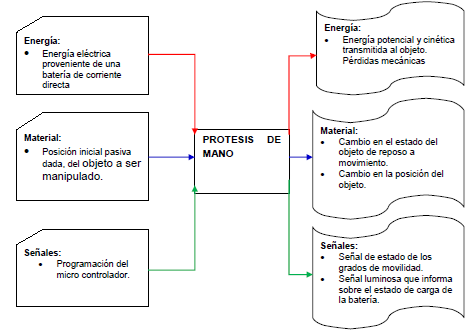
\includegraphics[width=100mm]{diagrama de la caja negra.png} % archivo
    \caption{Diagrama de la caja negra)\cite{ff5}.}
    \label{grafica:nueve}
\end{figure}

\textbf{Búsqueda Externa.} 


El siguiente punto es la concerniente a la búsqueda externa, en esta se aconseja realizar una serie de actividades encaminadas hacia la consecución de datos de usuarios líderes, expertos en el campo de la investigación correspondiente, consulta de patentes relacionadas y literatura existente, además de analizar los productos de la competencia\cite{ff5}.


Un ejemplo de esto podría ser.


o	I-Limb Hand (Figura 10). 

Características y prestaciones:
\\•	Agarre lateral. (Tarjetas, llaves).
\\•	Agarre cilíndrico.
\\•	Agarre fino.
\\•	Agarre esférico.
\\•	Agarre seguro en forma de gancho.
\\•	Permite prensión palmar.
\\•	Independencia de movimiento del dedo índice (Indicador).
\\•	Prono-supinación (Rotación del antebrazo).
\\•	Flexión y extensión de la muñeca.
\\•	Voltaje nominal: 7.5 V.
\\•	Corriente Nominal: 5 Amp.
\\•	Fuerza del índice al pulgar para prensión en las yemas de los dedos: 1.1 Kg.
\\•	Fuerza de pellizco lateral: 1.8-2 Kg.
\\•	Fuerza de prensión palmar: 8-9.5 Kg.
\\•	Limites de carga: 8.5-22 Kg.
\\•	Batería Recargable.
\\•	Peso entre 430 y 518 Gr dependiendo del tamaño\cite{ff5}.

\begin{figure}[H] % figura
    \centering
    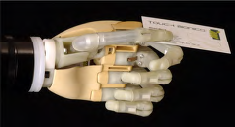
\includegraphics[width=100mm]{I-Limb Hand.png} % archivo
    \caption{I-Limb Hand)\cite{ff5}.}
    \label{grafica:diez}
\end{figure}

\textbf{Búsqueda interna.} 


1. Suspender Juicio.
\\2. Generar muchas ideas.
\\3. Dar la bienvenida a ideas que puedan ser no factibles.
\\4. Usar medios gráficos y físicos.
\\5. Estas directrices pueden ser usadas por personas que trabajen tanto en forma
individual como en grupos multidisciplinarios.
\\En este punto se deben iniciar a realizar los bocetos y a implementar las ideas anteriormente vistos ya sea a lápiz o en diferentes Softwares de diseño\cite{ff5}.

\begin{figure}[H] % figura
    \centering
    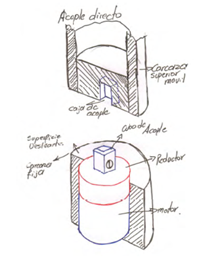
\includegraphics[width=80mm]{boceto.png} % archivo
    \caption{Boceto\cite{ff5}.}
    \label{grafica:once}
\end{figure}

\textbf{Filtrado de conceptos.} 


Este método para llegar al Concepto General de Diseño (CGD) está basado en uno que inicialmente fue desarrollado por Stuart Pugh en la década de los 80. El fin de esta etapa es reducir rápidamente el número de conceptos hasta llegar a uno particular el cual será desarrollado y mejorado. Los pasos propuestos en el método para llegar a este objetivo son:
\\o	Elaborar la o las matrices de selección según sea el caso.
\\o	Calificar los conceptos.
\\o	Evaluar los conceptos.
\\o	Combinar y mejorar los conceptos.
\\o	Seleccionar uno o más conceptos.
\\o	Meditar sobre los resultados y el proceso\cite{ff5}.


Las matrices de selección se construyeron agrupando las soluciones propuestas en tres grupos, de acuerdo a un criterio de proximidad de los sistemas y de trabajo complementario.
Así los grupos propuestos son:


o	Conjunto dedos-pulgar-palma.
\\o	Conjunto rotador muñeca.
\\o	Conjunto carcasa-acople muñón.


Básicamente en este paso es donde debemos pasar a desarrollar un diseño final con todas las mejoras y observaciones vistas anteriormente, a este diseño es al que se le dará vida una vez finalizado el proyecto\cite{ff5}.


\begin{figure}[H] % figura
    \centering
    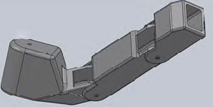
\includegraphics[width=80mm]{avance de prototipo.png} % archivo
    \caption{Avance de prototipo\cite{ff5}}
    \label{grafica:doce}
\end{figure}

\textbf{Evaluación de la prótesis para fabricación.} 


Se debe realizar una evaluación donde se vean todos los puntos y preparar el diseño final para su manufactura y elaboración física, en este proceso se deben ver todos los pro y los contra de el diseño una vez realizados los estudios de resistencia, las simulaciones de funcionamiento etc.
Una vez teniendo toda esta evaluación se puede proceder con el desarrollo físico y el ensamblaje de la prótesis\cite{ff5}.

\begin{figure}[H] % figura
    \centering
    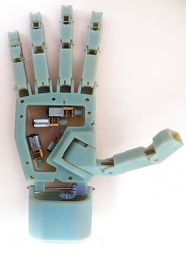
\includegraphics[width=80mm]{resultado final de la protesis.png} % archivo
    \caption{Resultado final de la prótesis\cite{ff5}}
    \label{grafica:trece}
\end{figure}


\section{Conclusiones}
Cada año la tecnología va cambiando para bien a favor del hombre, como son en este caso las prótesis, anteriormente era muy difícil tener una y aparte el cómo adaptarse a esta, ya que se tenía que cumplir con ciertos requisitos para ser uno de los seleccionados, la tecnología que se maneja hoy en día, nos ayuda a que sea más fácil el poder contar con una, en este tema se aprendió el cómo estas funcionan y los mecanismos que se utilizan para que tengan  un mejor manejo, un factor importante en este es las simulaciones, ya que este nos ayuda a comprobar que las prótesis estén bien diseñadas, ya que ahí es donde podemos llegar a detectar un error (si en dado caso se llagara a presentar).
Este tipo de actividades a nosotros como futuros ingenieros nos ayuda a poder ver un poco más allá estábamos tan acostumbrados a solo investigar sobre maquinas, simulaciones mecánicas y ahora empezar a conocer la anatomía de la mano saber que hay muchos tipos de prótesis, hace unos años conocí a un ingeniero en mecatrónica que estaba especializado en biodispositivos y tenía prototipos de prótesis para las venas del corazón eran unas prótesis tan chiquitas que quede asombrada de como el hombre puede crear infinidad de cosas para adaptarse a la vida diaria.



\bibliography{bib}
\bibliographystyle{plainnat}

\end{document}
